\documentclass[tikz,border=8pt]{standalone}
% Shared look for every TikZ diagram. Load with % Shared look for every TikZ diagram. Load with % Shared look for every TikZ diagram. Load with \input{../../tools/tikz-style.tex}
\usepackage[T1]{fontenc}
\usepackage{lmodern}
\renewcommand{\sfdefault}{lmr}  % diagrams use the same serif as the text
\usetikzlibrary{arrows.meta, positioning, shapes.geometric, calc, fit, backgrounds}
\definecolor{cblue}{HTML}{4C78A8}
\definecolor{corange}{HTML}{F58518}
\definecolor{cgreen}{HTML}{54A24B}
\definecolor{cred}{HTML}{E45756}
\definecolor{cpurple}{HTML}{B279A2}
\definecolor{cgrey}{HTML}{6B6B6B}
\tikzset{
  every picture/.style={font=\sffamily, line width=1.2pt},
  box/.style={draw=#1, fill=#1!12, rounded corners=4pt, align=center, inner sep=7pt, minimum height=1.1cm},
  box/.default=cgrey,
  arrow/.style={-{Stealth[length=3mm]}, draw=cgrey, line width=1.4pt},
  title/.style={font=\sffamily\bfseries\Large},
  note/.style={font=\sffamily\small, text=cgrey, align=center},
}
\AtBeginDocument{\hyphenpenalty=10000 \exhyphenpenalty=10000}

\usepackage[T1]{fontenc}
\usepackage{lmodern}
\renewcommand{\sfdefault}{lmr}  % diagrams use the same serif as the text
\usetikzlibrary{arrows.meta, positioning, shapes.geometric, calc, fit, backgrounds}
\definecolor{cblue}{HTML}{4C78A8}
\definecolor{corange}{HTML}{F58518}
\definecolor{cgreen}{HTML}{54A24B}
\definecolor{cred}{HTML}{E45756}
\definecolor{cpurple}{HTML}{B279A2}
\definecolor{cgrey}{HTML}{6B6B6B}
\tikzset{
  every picture/.style={font=\sffamily, line width=1.2pt},
  box/.style={draw=#1, fill=#1!12, rounded corners=4pt, align=center, inner sep=7pt, minimum height=1.1cm},
  box/.default=cgrey,
  arrow/.style={-{Stealth[length=3mm]}, draw=cgrey, line width=1.4pt},
  title/.style={font=\sffamily\bfseries\Large},
  note/.style={font=\sffamily\small, text=cgrey, align=center},
}
\AtBeginDocument{\hyphenpenalty=10000 \exhyphenpenalty=10000}

\usepackage[T1]{fontenc}
\usepackage{lmodern}
\renewcommand{\sfdefault}{lmr}  % diagrams use the same serif as the text
\usetikzlibrary{arrows.meta, positioning, shapes.geometric, calc, fit, backgrounds}
\definecolor{cblue}{HTML}{4C78A8}
\definecolor{corange}{HTML}{F58518}
\definecolor{cgreen}{HTML}{54A24B}
\definecolor{cred}{HTML}{E45756}
\definecolor{cpurple}{HTML}{B279A2}
\definecolor{cgrey}{HTML}{6B6B6B}
\tikzset{
  every picture/.style={font=\sffamily, line width=1.2pt},
  box/.style={draw=#1, fill=#1!12, rounded corners=4pt, align=center, inner sep=7pt, minimum height=1.1cm},
  box/.default=cgrey,
  arrow/.style={-{Stealth[length=3mm]}, draw=cgrey, line width=1.4pt},
  title/.style={font=\sffamily\bfseries\Large},
  note/.style={font=\sffamily\small, text=cgrey, align=center},
}
\AtBeginDocument{\hyphenpenalty=10000 \exhyphenpenalty=10000}

\begin{document}
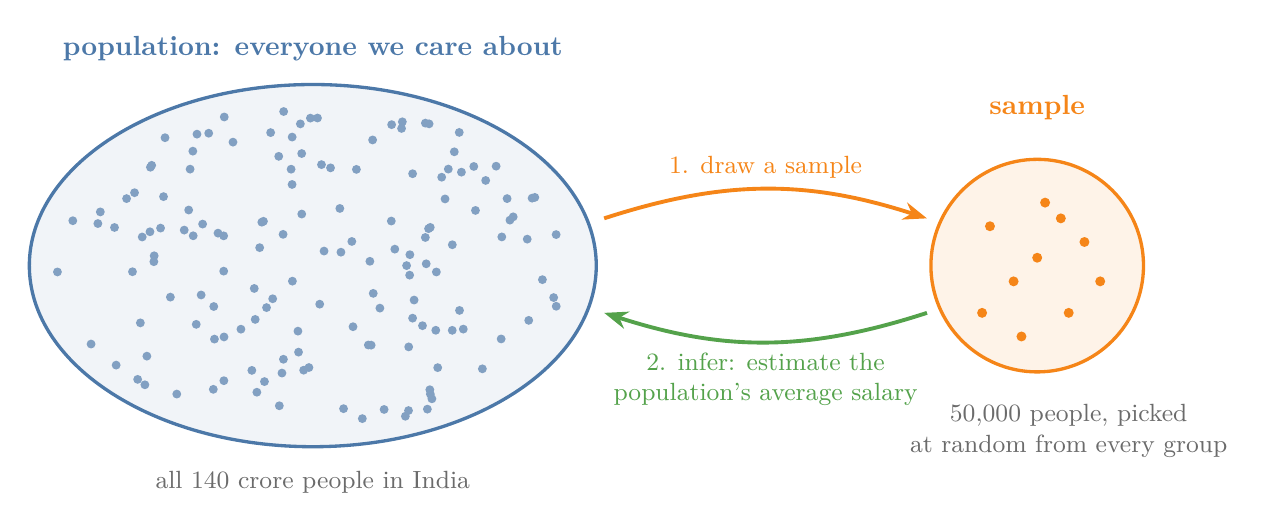
\begin{tikzpicture}
  % population: a big cloud of dots
  \node[draw=cblue, fill=cblue!8, ellipse, minimum width=7.2cm, minimum height=4.6cm] (pop) at (0,0) {};
  \pgfmathsetseed{7}
  \foreach \i in {1,...,150} {
    \pgfmathsetmacro{\a}{rnd*360}\pgfmathsetmacro{\r}{sqrt(rnd)}
    \fill[cblue!70] ({3.3*\r*cos(\a)},{2.05*\r*sin(\a)}) circle (1.6pt);
  }
  \node[font=\sffamily\bfseries, text=cblue] at (0,2.75) {population: everyone we care about};
  \node[note] at (0,-2.75) {all 140 crore people in India};
  % sample
  \node[draw=corange, fill=corange!10, circle, minimum size=2.7cm] (smp) at (9.2,0) {};
  \foreach \x/\y in {-0.6/0.5,0.1/0.8,0.6/0.3,-0.3/-0.2,0.4/-0.6,-0.7/-0.6,0.0/0.1,0.8/-0.2,-0.2/-0.9,0.3/0.6} {
    \fill[corange] (9.2+\x,\y) circle (1.8pt);
  }
  \node[font=\sffamily\bfseries, text=corange] at (9.2,2.0) {sample};
  \node[note] at (9.6,-2.1) {50{,}000 people, picked\\ at random from every group};
  \draw[arrow, draw=corange] (3.7,0.6) to[bend left=18] node[above, font=\sffamily\small, text=corange] {1. draw a sample} (7.8,0.6);
  \draw[arrow, draw=cgreen] (7.8,-0.6) to[bend left=18] node[below, font=\sffamily\small, text=cgreen, align=center] {2. infer: estimate the\\ population's average salary} (3.7,-0.6);
\end{tikzpicture}
\end{document}
